- numba benchmark code
    - comment on the programmer efficiency in simply decorating with Numba


\begin{figure}[!h]
    \centering
    {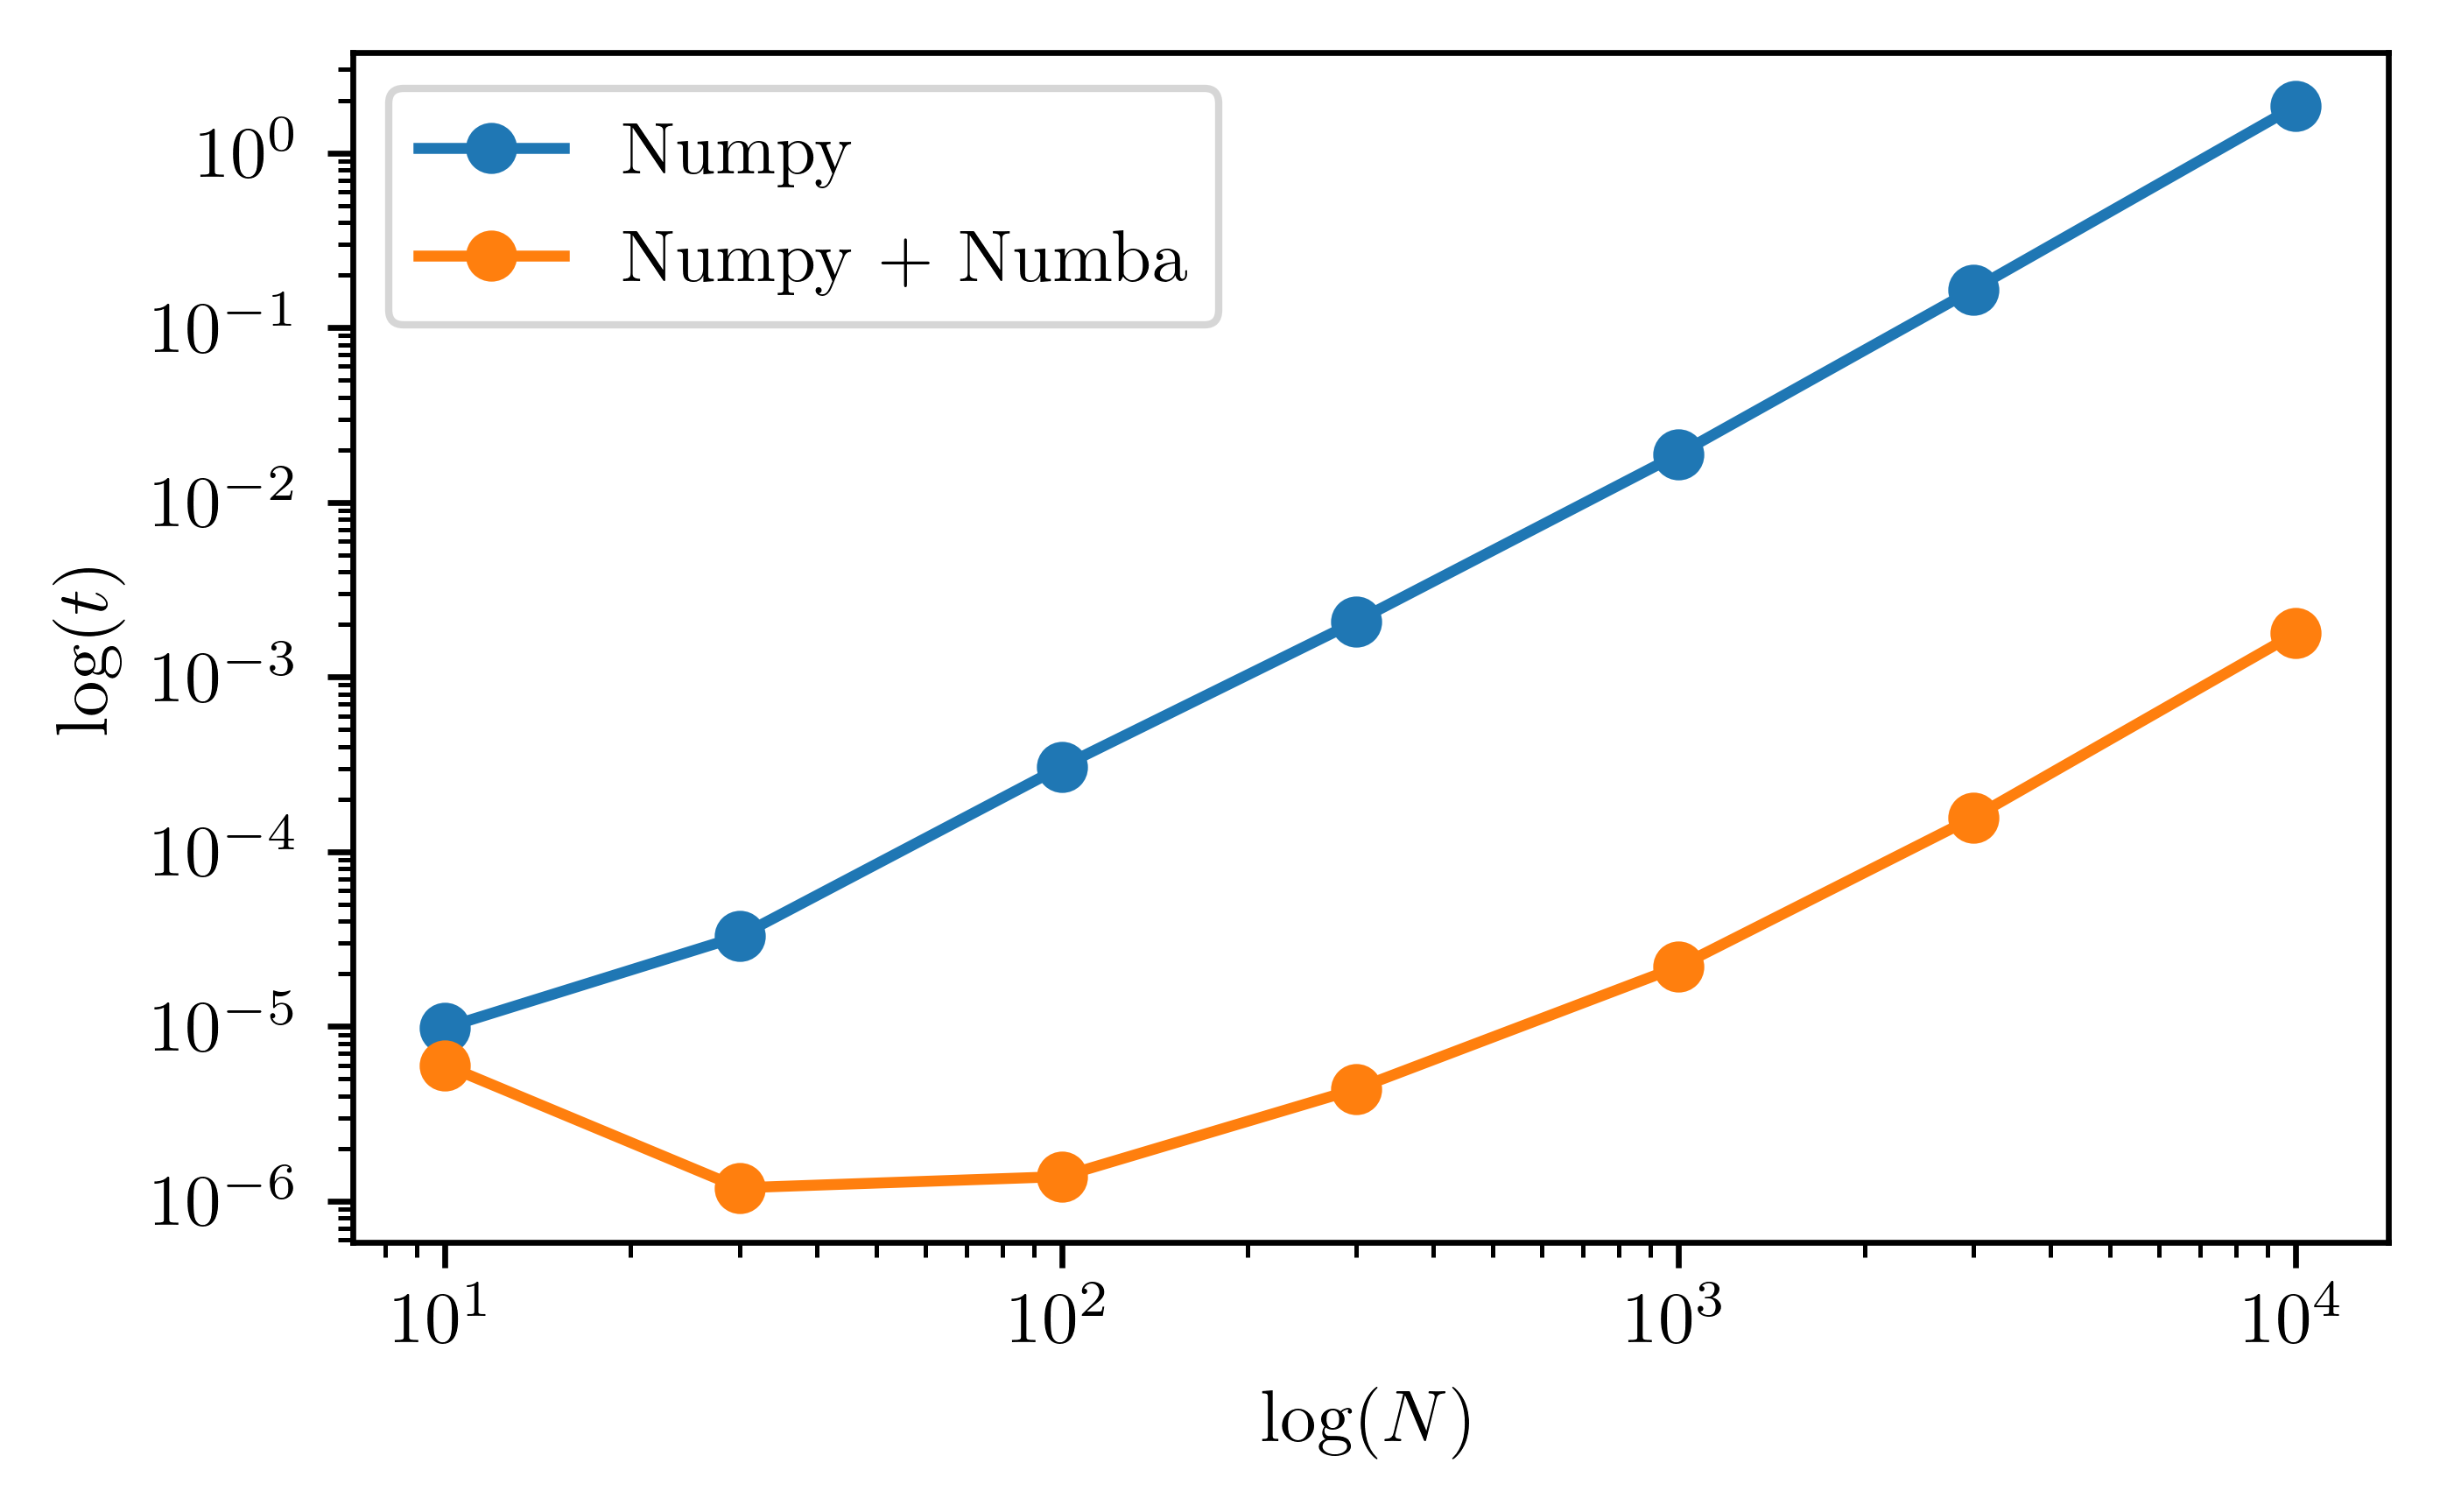
\includegraphics[width=\textwidth]{chapter3/numba.png}}

    \caption{foo bar}
    \label{fig:3_1_numba}
\end{figure}

- Estimate cost savings from each parallelization step
- numba
- hdf5 vs pickle
- multiproc

- Compare experimental results for FMM vs Direct computation as a function of number of particles for the LAPLACE KERNEL!!!!. Justify usage of laplace kernel (paradigm, easy etc.)

- [DIAGRAM] Need to plot the computational complexity.

- Understand cost of computation via pyexafmm compared to state of the art exafmm-t.

- Comment on where the slowness comes from

- no parallelism for operator evaluations

- no parallelism for memory sharing

- lots of copying of same data.

- subtoptimal data formats for m2l - lots of loading.

- suboptimal size of data structures lead to loading from non-cpu memory - which is slow - could be optimized via numexpr etc in the future or more intricate chunking of memory.

- These are justifiable from the time constraints on full-time development.

Figures required:

- KEY RESULT: Benchmarking figure as a function of N-particles
